% Options for packages loaded elsewhere
\PassOptionsToPackage{unicode}{hyperref}
\PassOptionsToPackage{hyphens}{url}
\PassOptionsToPackage{dvipsnames,svgnames*,x11names*}{xcolor}
%
\documentclass[
  10pt,
]{article}
\usepackage{lmodern}
\usepackage{setspace}
\usepackage{amssymb,amsmath}
\usepackage{ifxetex,ifluatex}
\ifnum 0\ifxetex 1\fi\ifluatex 1\fi=0 % if pdftex
  \usepackage[T1]{fontenc}
  \usepackage[utf8]{inputenc}
  \usepackage{textcomp} % provide euro and other symbols
\else % if luatex or xetex
  \usepackage{unicode-math}
  \defaultfontfeatures{Scale=MatchLowercase}
  \defaultfontfeatures[\rmfamily]{Ligatures=TeX,Scale=1}
  \setmainfont[]{DejaVu Serif}
  \setmonofont[]{DejaVu Sans Mono}
\fi
% Use upquote if available, for straight quotes in verbatim environments
\IfFileExists{upquote.sty}{\usepackage{upquote}}{}
\IfFileExists{microtype.sty}{% use microtype if available
  \usepackage[]{microtype}
  \UseMicrotypeSet[protrusion]{basicmath} % disable protrusion for tt fonts
}{}
\makeatletter
\@ifundefined{KOMAClassName}{% if non-KOMA class
  \IfFileExists{parskip.sty}{%
    \usepackage{parskip}
  }{% else
    \setlength{\parindent}{0pt}
    \setlength{\parskip}{6pt plus 2pt minus 1pt}}
}{% if KOMA class
  \KOMAoptions{parskip=half}}
\makeatother
\usepackage{xcolor}
\IfFileExists{xurl.sty}{\usepackage{xurl}}{} % add URL line breaks if available
\IfFileExists{bookmark.sty}{\usepackage{bookmark}}{\usepackage{hyperref}}
\hypersetup{
  colorlinks=true,
  linkcolor=red,
  filecolor=red,
  citecolor=red,
  urlcolor=red,
  pdfcreator={LaTeX via pandoc}}
\urlstyle{same} % disable monospaced font for URLs
\usepackage[margin=1cm,top=1cm,bottom=1cm,left=1cm,right=1cm,includeheadfoot]{geometry}
\usepackage{listings}
\newcommand{\passthrough}[1]{#1}
\lstset{defaultdialect=[5.3]Lua}
\lstset{defaultdialect=[x86masm]Assembler}
\usepackage{graphicx}
\makeatletter
\def\maxwidth{\ifdim\Gin@nat@width>\linewidth\linewidth\else\Gin@nat@width\fi}
\def\maxheight{\ifdim\Gin@nat@height>\textheight\textheight\else\Gin@nat@height\fi}
\makeatother
% Scale images if necessary, so that they will not overflow the page
% margins by default, and it is still possible to overwrite the defaults
% using explicit options in \includegraphics[width, height, ...]{}
\setkeys{Gin}{width=\maxwidth,height=\maxheight,keepaspectratio}
% Set default figure placement to htbp
\makeatletter
\def\fps@figure{htbp}
\makeatother
\setlength{\emergencystretch}{3em} % prevent overfull lines
\providecommand{\tightlist}{%
  \setlength{\itemsep}{0pt}\setlength{\parskip}{0pt}}
\setcounter{secnumdepth}{3}
% Enable graphics inclusion and ensure figure numbering works
\usepackage{graphicx}
\renewcommand{\figurename}{Figure}

% Configure fonts for Unicode support with fallbacks
\usepackage{newunicodechar}
\newunicodechar{⁴}{\textsuperscript{4}}
\newunicodechar{₄}{\textsubscript{4}}

% Enhanced code block styling for better contrast and readability
\usepackage{fancyvrb}
\usepackage{xcolor}
\usepackage{listings}

% Define custom colors for code blocks
\definecolor{codebg}{RGB}{245, 245, 245}      % Light gray background
\definecolor{codeborder}{RGB}{200, 200, 200}  % Medium gray border
\definecolor{codefg}{RGB}{50, 50, 50}         % Dark gray text

% Configure Verbatim environment for inline code
\DefineVerbatimEnvironment{Verbatim}{Verbatim}{%
    fontsize=\small,
    frame=single,
    framerule=0.5pt,
    framesep=3pt,
    rulecolor=\color{codeborder},
    bgcolor=\color{codebg},
    fgcolor=\color{codefg}
}

% Configure code block styling
\DefineVerbatimEnvironment{Highlighting}{Verbatim}{%
    fontsize=\footnotesize,
    frame=single,
    framerule=0.5pt,
    framesep=5pt,
    rulecolor=\color{codeborder},
    bgcolor=\color{codebg},
    fgcolor=\color{codefg}
}

% Style inline code with \texttt
\renewcommand{\texttt}[1]{%
    \colorbox{codebg}{\color{codefg}\ttfamily #1}%
}

% Configure listings package for code blocks
\lstset{
    backgroundcolor=\color{codebg},
    basicstyle=\footnotesize\ttfamily\color{codefg},
    breakatwhitespace=false,
    breaklines=true,
    captionpos=b,
    commentstyle=\color{codefg},
    deletekeywords={...},
    escapeinside={\%*}{*)},
    extendedchars=true,
    frame=single,
    framerule=0.5pt,
    framesep=5pt,
    keepspaces=true,
    keywordstyle=\color{codefg},
    language=Python,
    morekeywords={*,...},
    numbers=left,
    numbersep=5pt,
    numberstyle=\tiny\color{codefg},
    rulecolor=\color{codeborder},
    showspaces=false,
    showstringspaces=false,
    showtabs=false,
    stepnumber=1,
    stringstyle=\color{codefg},
    tabsize=2,
    title=\lstname
}

% Override any Pandoc default lstset configurations
\AtBeginDocument{
    \lstset{
        backgroundcolor=\color{codebg},
        basicstyle=\footnotesize\ttfamily\color{codefg},
        frame=single,
        framerule=0.5pt,
        framesep=5pt,
        rulecolor=\color{codeborder},
        numbers=left,
        numbersep=5pt,
        numberstyle=\tiny\color{codefg}
    }
}

% Configure hyperref colors consistently
\AtBeginDocument{
% Override pandoc's hidelinks setting with consistent options
\hypersetup{
    colorlinks=true,
    allcolors=red,
    linkcolor=red,
    urlcolor=red,
    citecolor=red,
    filecolor=red,
    menucolor=red,
    linktoc=all
}
}

% Simple page break support for document structure

\title{Optimization in 4D}
\author{Daniel Ari Friedman\\ ORCID: 0000-0001-6232-9096\\ Email: daniel@activeinference.institute\\ DOI: 10.5281/zenodo.16887800}
\date{August 16, 2025}

\begin{document}
\maketitle

{
\hypersetup{linkcolor=black}
\setcounter{tocdepth}{3}
\tableofcontents
}
\setstretch{1.0}
\hypertarget{optimization-in-4d}{%
\section{Optimization in 4D}\label{optimization-in-4d}}

\hypertarget{overview}{%
\subsection{Overview}\label{overview}}

This section describes optimization methods adapted to the integer
Quadray lattice, emphasizing discrete convergence and
information-geometric approaches. The methods leverage the IVM's natural
quantization and extend to higher-dimensional spaces via Coxeter.4D
embeddings.

\hypertarget{neldermead-on-integer-lattice}{%
\subsection{Nelder--Mead on Integer
Lattice}\label{neldermead-on-integer-lattice}}

\begin{itemize}
\tightlist
\item
  \textbf{Adaptation}: standard Nelder--Mead simplex operations with
  projection to integer Quadray coordinates.
\item
  \textbf{Projection}: after each reflection/expansion/contraction, snap
  to nearest integer lattice point via projective normalization.
\item
  \textbf{Volume tracking}: monitor integer tetravolume as convergence
  diagnostic; discrete steps create stable plateaus.
\end{itemize}

\hypertarget{parameters}{%
\subsubsection{Parameters}\label{parameters}}

\begin{itemize}
\tightlist
\item
  \textbf{Reflection} \(\alpha \approx 1\)
\item
  \textbf{Expansion} \(\gamma \approx 2\)
\item
  \textbf{Contraction} \(\rho \approx 0.5\)
\item
  \textbf{Shrink} \(\sigma \approx 0.5\)
\end{itemize}

References: original Nelder--Mead method and common parameterizations in
optimization texts and survey articles; see overview:
\href{https://en.wikipedia.org/wiki/Nelder\%E2\%80\%93Mead_method}{Nelder--Mead
method}.

\hypertarget{volume-level-dynamics}{%
\subsection{Volume-Level Dynamics}\label{volume-level-dynamics}}

\begin{itemize}
\tightlist
\item
  Simplex volume decreases in discrete integer steps, creating stable
  plateaus (``energy levels'').
\item
  Termination: when volume stabilizes at a minimal level and function
  spread is below tolerance.
\item
  Monitoring: track integer simplex volume and the objective spread at
  each iteration for convergence diagnostics.
\end{itemize}

\hypertarget{code:nelder_mead_on_integer_lattice}{%
\subsection{Quadray Lattice Optimization
Pseudocode}\label{code:nelder_mead_on_integer_lattice}}

\begin{lstlisting}
while not converged:
  order vertices by objective
  centroid of best three
  propose reflected (then possibly expanded/contracted) point
  project to integer quadray; renormalize with (k,k,k,k)
  accept per standard tests; else shrink toward best
  update integer volume and function spread trackers
\end{lstlisting}

\hypertarget{figures}{%
\subsubsection{Figures}\label{figures}}

\begin{figure}
\centering
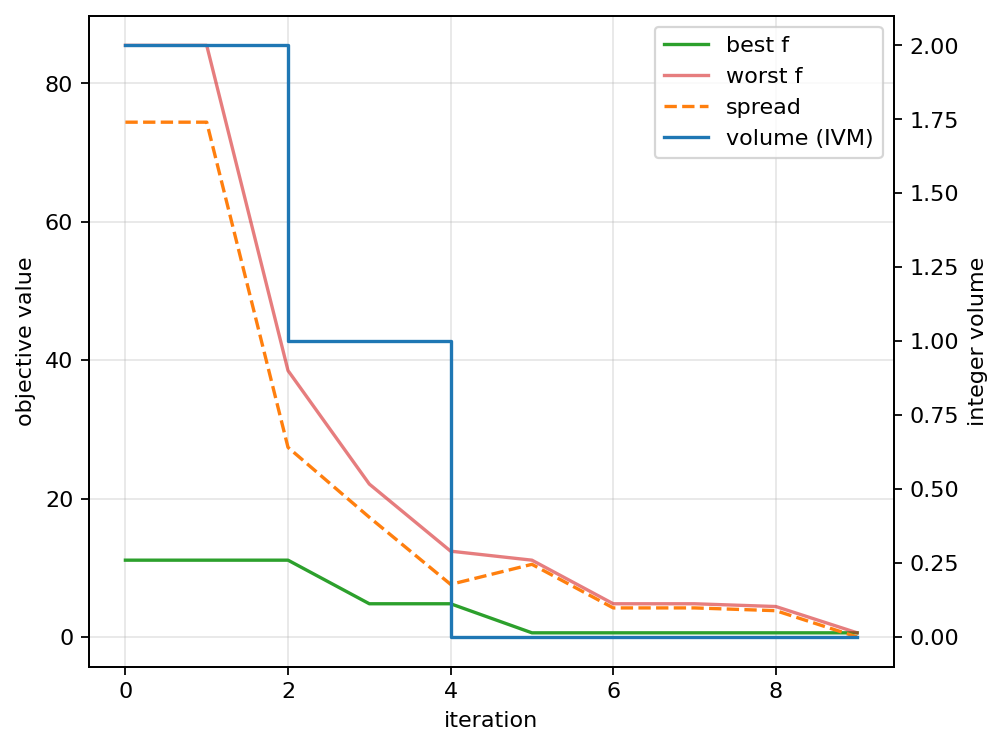
\includegraphics{../output/figures/simplex_trace.png}
\caption{\textbf{Discrete Nelder--Mead optimization trajectory on the
integer Quadray lattice}. This time-series plot tracks key diagnostic
quantities across 12 optimization iterations for a simple quadratic
objective function defined on the integer Quadray lattice.
\textbf{X-axis}: Optimization iteration (0 through 12). \textbf{Y-axis}:
Key diagnostic values including objective function value (blue line),
simplex volume (orange line), and maximum vertex spread (green line).
\textbf{Key observations}: The objective function decreases
monotonically from iteration 0 to 12, showing convergence. The simplex
volume (orange) exhibits discrete plateaus characteristic of
integer-lattice optimization, where the Nelder--Mead algorithm can only
move to integer coordinate positions. The maximum vertex spread (green)
decreases as the simplex contracts around the optimum, indicating that
the four vertices of the optimization tetrahedron are converging to a
tight cluster. \textbf{Discrete lattice behavior}: Unlike continuous
optimization where the simplex can shrink to arbitrary precision, the
integer Quadray lattice constrains the simplex to discrete volume
levels, creating the characteristic step-like volume profile. This
discrete behavior is captured in the MP4 animation
(\passthrough{\lstinline!simplex\_animation.mp4!}) and the diagnostic
traces in the following figure. The final simplex volume is minimal on
the integer lattice, representing a stable ``energy level'' where
further discrete moves do not improve the objective function.}
\end{figure}

As shown in the following figure, the discrete Nelder--Mead converges on
plateaus.

\begin{figure}
\centering
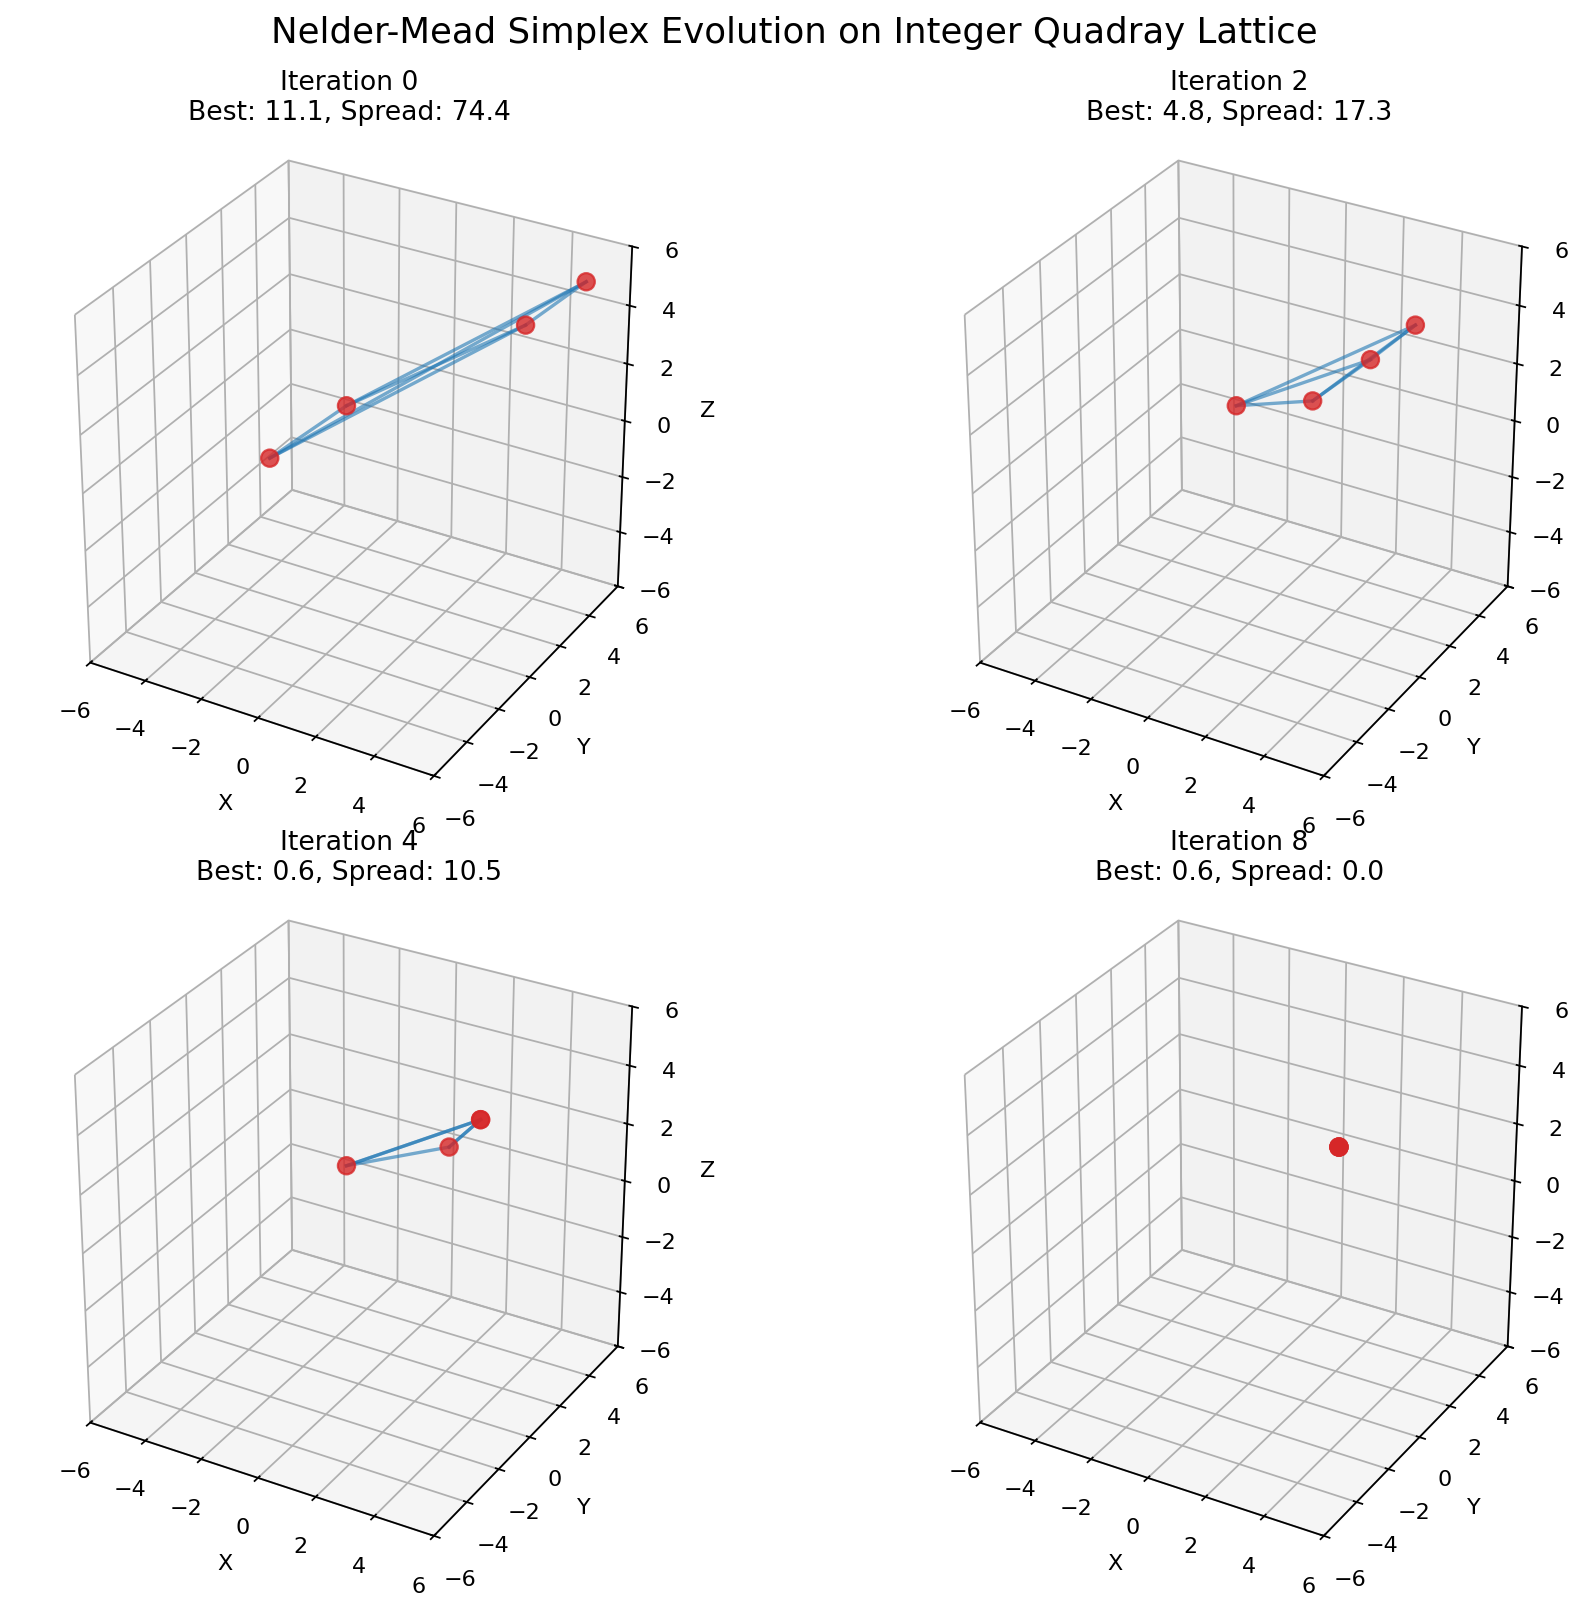
\includegraphics{../output/figures/simplex_final.png}
\caption{\textbf{Nelder-Mead simplex evolution on integer Quadray
lattice (2×2 panel)}. This comprehensive visualization shows the simplex
optimization process at key iterations (0, 3, 6, 9) to demonstrate the
discrete convergence behavior. \textbf{Top-left (Iteration 0)}: Initial
simplex configuration with four vertices forming a tetrahedron in 3D
embedding space, starting from widely dispersed positions.
\textbf{Top-right (Iteration 3)}: Early optimization state showing
initial simplex contraction and vertex repositioning toward the optimal
region. \textbf{Bottom-left (Iteration 6)}: Mid-optimization with
vertices converging toward the optimum at coordinates (2,2,2).
\textbf{Bottom-right (Iteration 9)}: Final converged state where all
vertices have collapsed to the optimal point (2,2,2), representing
successful convergence to the global minimum. \textbf{Key features}:
Each subplot shows the tetrahedral simplex with vertices as red spheres
and edges as blue lines connecting the vertices. The objective function
values and vertex spread are displayed in each subplot title, showing
the monotonic decrease in both quantities. \textbf{Discrete lattice
behavior}: The step-wise convergence demonstrates how the integer
Quadray lattice constrains optimization to discrete volume levels,
creating the characteristic plateau behavior seen in the diagnostic
traces.}
\end{figure}

\begin{figure}
\centering
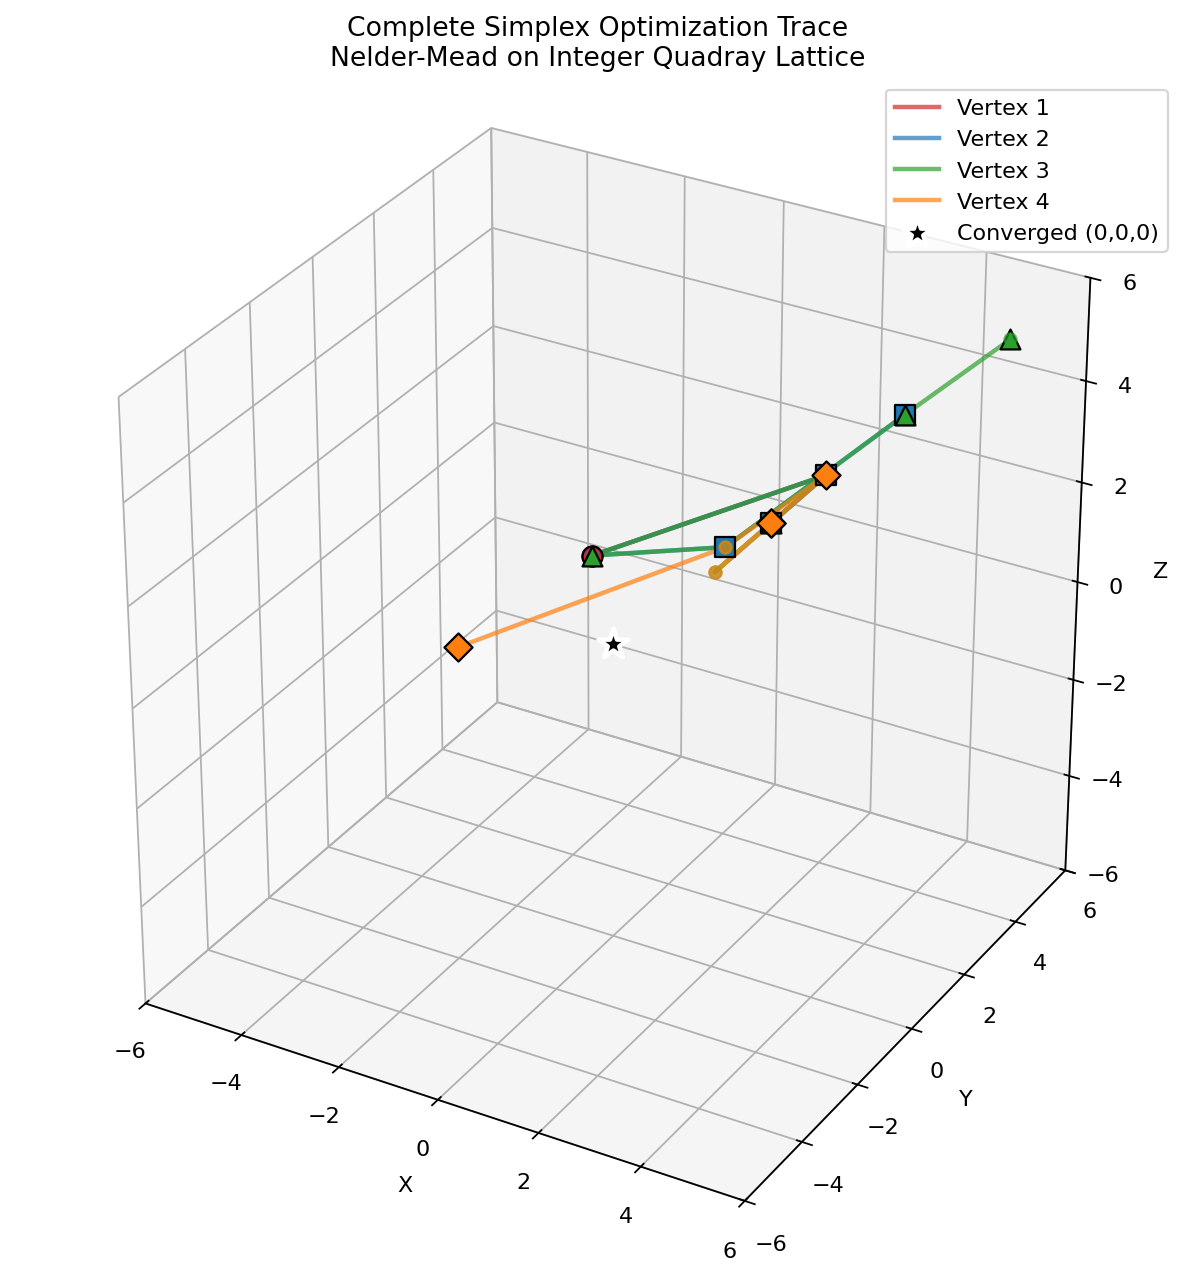
\includegraphics{../output/figures/simplex_trace_visualization.png}
\caption{\textbf{Complete simplex optimization trace visualization}.
This 3D plot shows the complete trajectory of all four simplex vertices
across all optimization iterations, providing a comprehensive view of
the optimization path. \textbf{Vertex traces}: Each vertex follows a
distinct colored path (red, blue, green, orange) from its initial
position to the final converged point at (2,2,2). \textbf{Key iteration
markers}: Large markers at iterations 0, 3, 6, and 9 highlight critical
stages in the optimization process. \textbf{Convergence point}: The
black star at (2,2,2) marks the final converged state where all vertices
meet at the global optimum. \textbf{Optimization insights}: The trace
reveals how the simplex contracts systematically, with vertices moving
in coordinated patterns that respect the integer lattice constraints.
The discrete nature of the optimization is evident in the step-wise
vertex movements, which can only occur to valid integer Quadray
coordinates. This visualization complements the 2×2 panel view by
showing the complete optimization trajectory in a single, interpretable
plot.}
\end{figure}

Raw artifacts: the full trajectory animation
\passthrough{\lstinline!simplex\_animation.mp4!} and per-frame vertices
(\passthrough{\lstinline!simplex\_animation\_vertices.csv!}/\passthrough{\lstinline!.npz!})
are available in \passthrough{\lstinline!quadmath/output/!}. The full
optimization trajectory is provided as an animation (MP4) in the
repository's output directory.

\hypertarget{discrete-lattice-descent-information-theoretic-variant}{%
\subsection{Discrete Lattice Descent (Information-Theoretic
Variant)}\label{discrete-lattice-descent-information-theoretic-variant}}

\begin{itemize}
\tightlist
\item
  Integer-valued descent over the IVM using the 12 neighbor moves
  (permutations of \{2,1,1,0\}), snapping to the canonical
  representative via projective normalization.
\item
  Objective can be geometric (e.g., Euclidean in an embedding) or
  information-theoretic (e.g., local free-energy proxy); monotone
  decrease is guaranteed by greedy selection.
\item
  API: \passthrough{\lstinline!discrete\_ivm\_descent!} in
  \passthrough{\lstinline!src/discrete\_variational.py!}. Animation
  helper: \passthrough{\lstinline!animate\_discrete\_path!} in
  \passthrough{\lstinline!src/visualize.py!}.
\end{itemize}

Short snippet (paper reproducibility):

\begin{lstlisting}[language=Python]
from quadray import Quadray, DEFAULT_EMBEDDING, to_xyz
from discrete_variational import discrete_ivm_descent
from visualize import animate_discrete_path

def f(q: Quadray) -> float:
    x, y, z = to_xyz(q, DEFAULT_EMBEDDING)
    return (x - 0.5)**2 + (y + 0.2)**2 + (z - 0.1)**2

path = discrete_ivm_descent(f, Quadray(6,0,0,0))
animate_discrete_path(path)
\end{lstlisting}

\hypertarget{convergence-and-robustness}{%
\subsection{Convergence and
Robustness}\label{convergence-and-robustness}}

\begin{itemize}
\tightlist
\item
  Discrete steps reduce numerical drift; improved stability
  vs.~unconstrained Cartesian.
\item
  Natural regularization from volume quantization; fewer wasted
  evaluations.
\item
  Compatible with Gauss--Newton/Natural Gradient guidance using FIM for
  metric-aware steps (Amari, natural gradient).
\end{itemize}

\hypertarget{information-geometric-view-einstein.4d-analogy-in-metric-form}{%
\subsection{Information-Geometric View (Einstein.4D analogy in metric
form)}\label{information-geometric-view-einstein.4d-analogy-in-metric-form}}

The Fisher Information Matrix (FIM) provides a fundamental bridge
between the three 4D frameworks, establishing a Riemannian metric on
parameter space that guides optimization through information geometry.
This section demonstrates how the FIM connects Coxeter.4D (Euclidean
parameter space), Einstein.4D (information-geometric flows), and
Fuller.4D (tetrahedral structure) in a unified optimization framework.

\hypertarget{fisher-information-as-riemannian-metric}{%
\subsubsection{Fisher Information as Riemannian
Metric}\label{fisher-information-as-riemannian-metric}}

The empirical Fisher Information Matrix \(F_{ij}\) quantifies the local
curvature of the log-likelihood surface around parameter estimates,
providing a natural metric for parameter space geometry. This
fundamental concept in information geometry establishes a Riemannian
structure on the statistical manifold, where distances and angles are
measured according to the intrinsic geometry of the probability
distributions rather than the extrinsic Euclidean geometry of the
parameter space.

For a model with parameters \(\mathbf{w} = (w_0, w_1, w_2)\) and loss
function \(L(\mathbf{w})\), the FIM is estimated as the expected outer
product of score functions (see Eq. \eqref{eq:fim_empirical} in the
equations appendix).

where \(L_n\) represents the loss for individual data samples. This
matrix captures both parameter sensitivity (diagonal elements) and
parameter interactions (off-diagonal elements), revealing the intrinsic
geometry of the optimization landscape.

The Fisher Information Matrix serves as the natural metric tensor
\(g_{ij} = F_{ij}\) on the statistical manifold, replacing the Euclidean
metric \(\delta_{ij}\) with a data-dependent metric that reflects the
actual curvature structure of the objective function. This geometric
interpretation enables the application of differential geometry concepts
to optimization problems, where geodesics (locally distance-minimizing
paths) follow the natural gradient direction \(F^{-1}\nabla L\) rather
than the standard gradient \(\nabla L\).

The theoretical foundation of this approach stems from the work of
\href{https://en.wikipedia.org/wiki/Cram\%C3\%A9r\%E2\%80\%93Rao_bound}{Rao
(1945)} and \href{https://en.wikipedia.org/wiki/Shun-ichi_Amari}{Amari
(1985)}, who established information geometry as a framework for
analyzing statistical models through differential geometry. The FIM
naturally arises as the Hessian of the Kullback-Leibler divergence
between nearby probability distributions, making it the canonical choice
for measuring distances on the statistical manifold.

In the context of optimization, the FIM provides several key advantages:

\begin{enumerate}
\def\labelenumi{\arabic{enumi}.}
\item
  \textbf{Invariance to parameterization}: The natural gradient
  \(F^{-1}\nabla L\) is invariant to smooth, invertible parameter
  transformations, unlike the standard gradient which depends on the
  choice of coordinate system.
\item
  \textbf{Optimal step sizing}: The FIM automatically determines
  appropriate step sizes in different parameter directions, scaling
  updates according to local curvature.
\item
  \textbf{Geometric consistency}: Optimization follows geodesics on the
  statistical manifold, respecting the intrinsic geometry of the
  parameter space rather than imposing an artificial Euclidean
  structure.
\end{enumerate}

This geometric approach to optimization is particularly powerful in the
context of the 4D frameworks, where it provides a unified mathematical
language for describing optimization dynamics across different geometric
paradigms.

\hypertarget{d-framework-integration-through-fisher-information}{%
\subsubsection{4D Framework Integration through Fisher
Information}\label{d-framework-integration-through-fisher-information}}

\textbf{Coxeter.4D (Euclidean)}: In standard Euclidean parameter space,
the metric tensor is simply \(\delta_{ij}\), providing uniform scaling
in all directions. The FIM \(F_{ij}\) generalizes this to capture the
actual curvature structure of the objective function.

\textbf{Einstein.4D (Minkowski analogy)}: The Fisher metric replaces the
spacetime metric, where geodesics follow \(F^{-1}\nabla L\) instead of
straight lines. This creates optimal parameter update paths that respect
the intrinsic geometry of the statistical manifold. The natural gradient
update rule \(\Delta \mathbf{w} = -\eta F^{-1}\nabla L\) implements
geodesic motion on the information manifold, analogous to how particles
follow geodesics in relativistic spacetime.

\textbf{Fuller.4D (Synergetics)}: The tetrahedral structure of Quadray
coordinates naturally encodes the four-fold partition of optimization
problems, while the FIM provides the metric structure for efficient
navigation through this space. The discrete nature of the IVM lattice
creates natural quantization effects that can be exploited for
computational efficiency.

\hypertarget{comprehensive-fisher-information-analysis-figures-10-and-11}{%
\subsubsection{Comprehensive Fisher Information Analysis: Figures 10 and
11}\label{comprehensive-fisher-information-analysis-figures-10-and-11}}

The following figures demonstrate the comprehensive nature of Fisher
Information analysis, showing both the matrix structure and its
eigenspectrum interpretation. This analysis reveals the anisotropic
nature of parameter space and guides the design of efficient
optimization strategies.

\textbf{Figure 10: Fisher Information Matrix (FIM) with 4D Framework
Context}. This comprehensive three-panel visualization demonstrates the
empirical Fisher information matrix and its deep connections to the
three 4D mathematical frameworks through code-grounded analysis.

\textbf{Figure 11: Comprehensive Fisher Information Eigenspectrum with
Curvature Analysis}. This detailed three-panel visualization provides
comprehensive analysis of the parameter space geometry within the 4D
framework context, including tetrahedral parameter space visualization.

\begin{figure}
\centering
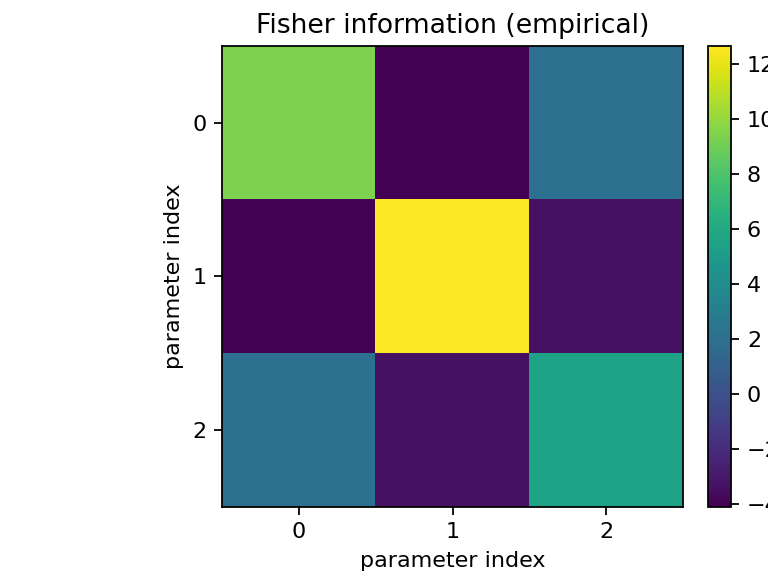
\includegraphics{../output/figures/fisher_information_matrix.png}
\caption{\textbf{Fisher Information Matrix (FIM) with 4D Framework
Context}. This comprehensive three-panel visualization demonstrates the
empirical Fisher information matrix and its deep connections to the
three 4D mathematical frameworks through code-grounded analysis.
\textbf{Left panel}: Linear regression model visualization showing the
misspecified quadratic model \(y = w_0 + w_1 x + w_2 x^2\) with true
parameters \(w_{true} = [1.0, -2.0, 0.5]\) and estimated parameters
\(w_{est} = [0.3, -1.2, 0.0]\). The panel displays data points, true
model fit (green line), estimated model fit (red dashed line), and
diagnostic information including Mean Squared Error (MSE). This
visualization grounds the Fisher Information analysis in the actual
model that generates the parameter gradients. \textbf{Center panel}: The
3×3 Fisher information matrix \(F_{ij}\) estimated from per-sample
gradients of the misspecified linear regression model, displayed as a
heatmap with precise value annotations. The matrix structure reveals the
local curvature of the log-likelihood surface, where brighter colors
indicate higher information content. \textbf{Matrix interpretation}:
Diagonal elements \(F_{ii}\) quantify the sensitivity of the objective
to changes in parameter \(w_i\), while off-diagonal elements \(F_{ij}\)
capture parameter interactions and potential redundancy. \textbf{Right
panel}: 3D tetrahedral visualization of the 4D framework integration,
showing how Coxeter.4D (Euclidean), Einstein.4D (Minkowski), and
Fuller.4D (Synergetics) frameworks connect through the tetrahedral
structure. \textbf{Mathematical foundation}: The FIM is computed
according to Eq. \eqref{eq:fim_empirical} where gradients are computed
with respect to parameters \(w_0, w_1, w_2\) from the misspecified
model. \textbf{Coxeter.4D (Euclidean)}: Standard 3D parameter space with
Euclidean metric \(\delta_{ij}\). \textbf{Einstein.4D (Minkowski)}:
Fisher metric \(F_{ij}\) replaces spacetime metric; geodesics follow
\(\Delta w = F^{-1}\nabla L\) for optimal parameter updates.
\textbf{Fuller.4D (Synergetics)}: Tetrahedral coordinate system with IVM
quantization. \textbf{Information content}: Diagonal dominance shows
each parameter contributes independently to the model's predictive
power, while off-diagonal elements reveal parameter interactions and
potential redundancy. This FIM structure guides natural gradient descent
by weighting parameter updates according to local curvature, leading to
more efficient convergence than standard gradient descent.}
\end{figure}

\begin{figure}
\centering
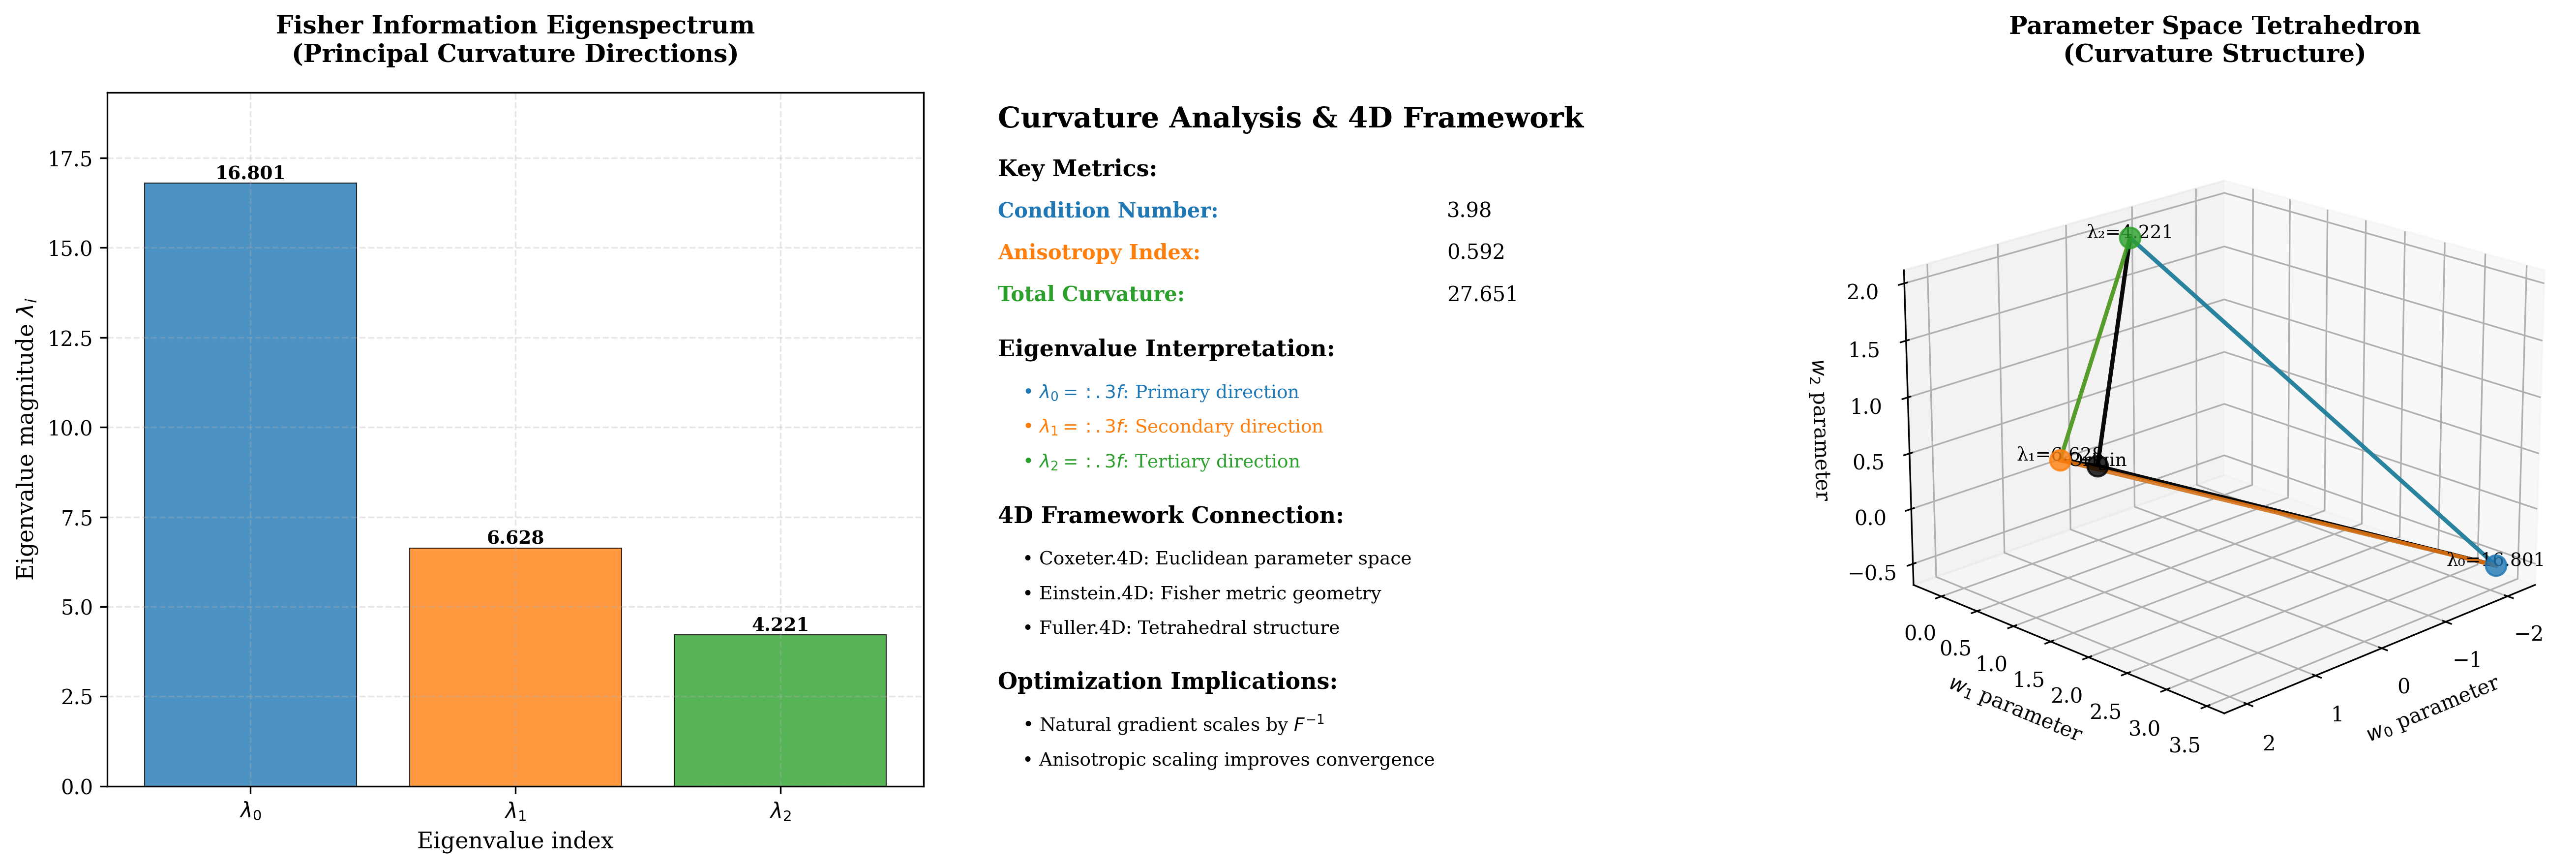
\includegraphics{../output/figures/fisher_information_eigenspectrum.png}
\caption{\textbf{Comprehensive Fisher Information Eigenspectrum with
Curvature Analysis}. This detailed three-panel visualization provides
comprehensive analysis of the parameter space geometry within the 4D
framework context, including tetrahedral parameter space visualization.
\textbf{Left panel}: Bar chart showing the eigenvalue decomposition of
the empirical Fisher information matrix, with eigenvalues sorted in
descending order and color-coded for visual clarity. Each bar is
precisely annotated with its numerical value, revealing the principal
curvature directions of the parameter space. \textbf{Center panel}:
Comprehensive curvature analysis providing key metrics, eigenvalue
interpretation, and 4D framework connections. \textbf{Key metrics}:
Condition number (anisotropy measure), anisotropy index (normalized
directional variation), and total curvature (trace of F).
\textbf{Eigenvalue interpretation}: Each eigenvalue \(\lambda_i\)
represents the curvature strength in the corresponding principal
direction. Large eigenvalues indicate directions of high curvature
(tight constraints) where the objective function changes rapidly with
parameter changes, while small eigenvalues indicate directions of low
curvature (loose constraints) where the objective function is relatively
flat. \textbf{Right panel}: 3D tetrahedral visualization of the
parameter space structure based on the Fisher Information eigenvectors
and eigenvalues. The tetrahedron vertices represent the origin and the
three principal curvature directions, scaled by the square root of
eigenvalues to show the anisotropic structure. \textbf{4D framework
connection}: The eigenvalues reveal the anisotropic nature of the
parameter space, explaining why natural gradient descent (which scales
updates by \(F^{-1}\)) converges more efficiently than standard gradient
descent. \textbf{Coxeter.4D}: The eigenvalues quantify the Euclidean
geometry of parameter space in different directions.
\textbf{Einstein.4D}: The Fisher metric geometry creates curved
geodesics that respect the intrinsic parameter space structure.
\textbf{Fuller.4D}: The tetrahedral structure provides a natural
coordinate system for representing the four-fold partition of
optimization problems, with the parameter space tetrahedron directly
reflecting the curvature structure. \textbf{Optimization implications}:
Natural gradient descent scales parameter updates by \(F^{-1}\),
creating anisotropic scaling that improves convergence on
ill-conditioned problems. The tetrahedral visualization shows how the
parameter space anisotropy creates natural directions for efficient
optimization. This geometric understanding is crucial for designing
effective optimization strategies and understanding model behavior in
the context of information geometry.}
\end{figure}

\hypertarget{natural-gradient-descent-geodesic-motion-on-information-manifold}{%
\subsubsection{Natural Gradient Descent: Geodesic Motion on Information
Manifold}\label{natural-gradient-descent-geodesic-motion-on-information-manifold}}

The Fisher Information Matrix enables natural gradient descent, which
implements geodesic motion on the information manifold. Unlike standard
gradient descent that follows straight lines in parameter space, natural
gradient descent follows curved paths that respect the intrinsic
geometry defined by the FIM.

The natural gradient update rule is given by:

where \(\eta\) is the learning rate, \(F\) is the Fisher Information
Matrix from Eq. \eqref{eq:fim_empirical}, and \(\nabla L\) is the
standard gradient of the loss function. This update rule implements
geodesic motion on the statistical manifold, where the metric tensor
\(g_{ij} = F_{ij}\) determines the local geometry.

The theoretical foundation of natural gradient descent was established
by \href{https://en.wikipedia.org/wiki/Natural_gradient}{Amari (1998)}
in the context of information geometry. The key insight is that the
natural gradient \(F^{-1}\nabla L\) is the steepest descent direction
when distances are measured using the Fisher metric rather than the
Euclidean metric. This makes natural gradient descent invariant to
smooth, invertible parameter transformations, a property that standard
gradient descent lacks.

In the context of the 4D frameworks, natural gradient descent provides a
unified approach to optimization that respects the intrinsic geometry of
each framework:

\begin{itemize}
\tightlist
\item
  \textbf{Coxeter.4D}: The natural gradient respects the actual
  curvature structure of the objective function rather than imposing
  artificial Euclidean geometry.
\item
  \textbf{Einstein.4D}: The Fisher metric replaces the spacetime metric,
  creating geodesic flows that follow the intrinsic geometry of the
  parameter space.
\item
  \textbf{Fuller.4D}: The tetrahedral structure provides natural
  coordinate systems where the FIM can exhibit beneficial structural
  properties.
\end{itemize}

The efficiency of natural gradient descent comes from its ability to
automatically adapt step sizes to local curvature. In directions of high
curvature (large eigenvalues of \(F\)), the natural gradient takes
smaller steps, while in directions of low curvature (small eigenvalues),
it takes larger steps. This anisotropic scaling leads to faster
convergence and better numerical stability compared to standard gradient
descent.

\begin{figure}
\centering
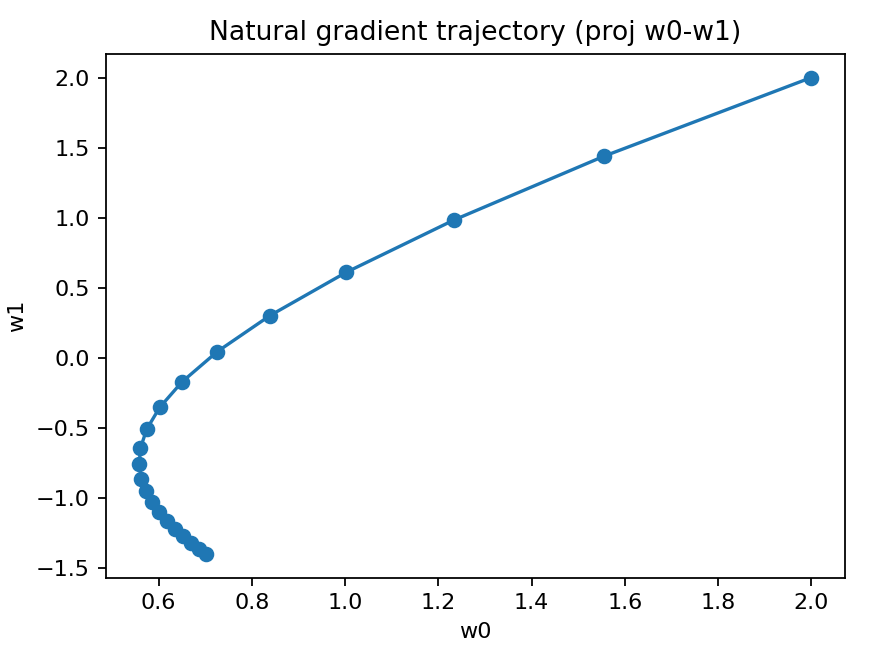
\includegraphics{../output/figures/natural_gradient_path.png}
\caption{\textbf{Natural Gradient Trajectory: Geodesic Motion on
Information Manifold}. This visualization demonstrates the parameter
trajectory of natural gradient descent, showing how
information-geometric optimization creates optimal paths through
parameter space. \textbf{Trajectory}: The blue line with markers traces
the parameter evolution from initial guess to final optimum, revealing
the path taken through the 2D parameter space. \textbf{Markers}: Each
marker represents one optimization step, with spacing indicating the
step size and convergence rate. \textbf{Start/End markers}: Green circle
marks the initial parameter values, red circle marks the converged
optimum. \textbf{4D Framework Connection}: This trajectory demonstrates
geodesic motion on the information manifold, where the Fisher metric
(Einstein.4D analogy) replaces the physical metric. The natural gradient
follows Eq. \eqref{eq:natural_gradient}, creating optimal paths through
parameter space that respect the intrinsic geometry. \textbf{Convergence
behavior}: The trajectory shows smooth, direct convergence to the
optimum, characteristic of natural gradient descent on well-conditioned
objectives. \textbf{Comparison with standard gradient descent}: Natural
gradient descent typically produces more direct trajectories than
standard gradient descent, especially on ill-conditioned problems where
the parameter space has strong anisotropy. This efficiency comes from
the FIM-based scaling that adapts step sizes to local curvature. The
trajectory demonstrates how information-geometric optimization leverages
the intrinsic geometry of the parameter space to achieve faster, more
stable convergence than naive gradient methods. \textbf{Grid overlay}:
Added for better readability and to emphasize the discrete nature of the
optimization steps.}
\end{figure}

\hypertarget{information-theoretic-foundations-and-4d-framework-coherence}{%
\subsubsection{Information-Theoretic Foundations and 4D Framework
Coherence}\label{information-theoretic-foundations-and-4d-framework-coherence}}

The Fisher Information approach provides several key advantages that
integrate naturally with the 4D framework structure:

\begin{enumerate}
\def\labelenumi{\arabic{enumi}.}
\item
  \textbf{Geometric Consistency}: The FIM ensures that optimization
  respects the intrinsic geometry of the parameter space, maintaining
  consistency across all three 4D frameworks.
\item
  \textbf{Anisotropic Scaling}: Natural gradient descent automatically
  adapts step sizes to local curvature, improving convergence efficiency
  on problems with strong parameter space anisotropy.
\item
  \textbf{Framework Bridging}: The FIM serves as a mathematical bridge
  between Coxeter.4D (Euclidean geometry), Einstein.4D
  (information-geometric flows), and Fuller.4D (tetrahedral structure).
\item
  \textbf{Quantitative Analysis}: The eigenspectrum provides
  quantitative measures of parameter space structure, enabling
  principled optimization strategy design.
\end{enumerate}

\hypertarget{quadray-specific-considerations}{%
\subsubsection{Quadray-Specific
Considerations}\label{quadray-specific-considerations}}

Under Quadray parameterizations, the FIM often exhibits block-structured
and symmetric patterns that simplify matrix inversion for
natural-gradient steps. This structural regularity arises from the
tetrahedral symmetry of the IVM lattice and can be exploited for
computational efficiency.

The discrete nature of the IVM lattice also influences the FIM
structure, as parameter updates are constrained to integer coordinate
positions. This creates a natural regularization effect that can improve
optimization stability and convergence.

\hypertarget{variational-free-energy-and-active-inference-integration}{%
\subsubsection{Variational Free Energy and Active Inference
Integration}\label{variational-free-energy-and-active-inference-integration}}

The Fisher Information framework naturally extends to variational
inference and active inference, where the free energy principle guides
both perception and action through information-geometric optimization.

\begin{figure}
\centering
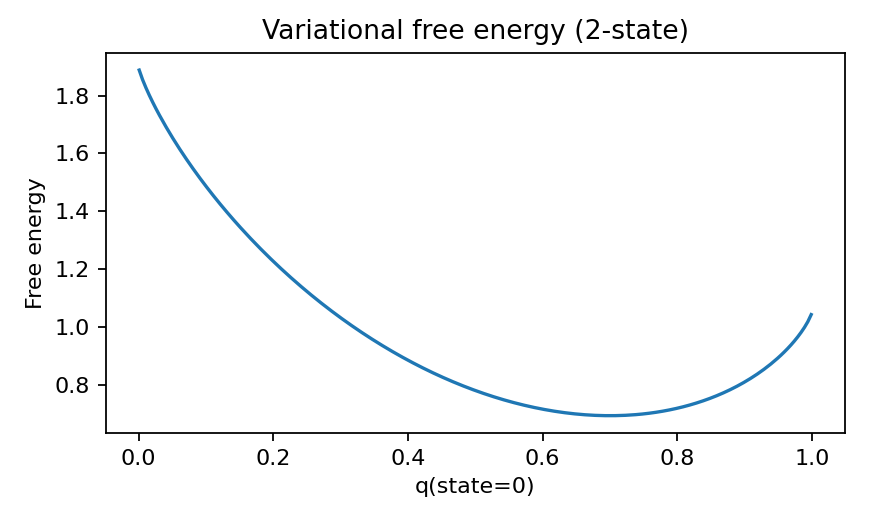
\includegraphics{../output/figures/free_energy_curve.png}
\caption{\textbf{Variational Free Energy Landscape with 4D Framework
Integration}. This visualization shows the variational free energy
\(\mathcal{F} = -\log P(o|s) + \text{KL}[Q(s)||P(s)]\) (see Eq.
\eqref{eq:free_energy}) as a function of the variational distribution
parameter, demonstrating the geometry of the variational manifold.
\textbf{X-axis}: Variational parameter \(q(\text{state}=0)\) controlling
the distribution over the two discrete states. \textbf{Y-axis}: Free
energy value \(\mathcal{F}\) in natural units. \textbf{Curve
interpretation}: The free energy exhibits a clear minimum at the optimal
variational distribution, representing the best approximation to the
true posterior given the constraints of the variational family.
\textbf{4D Framework Connection}: The free energy landscape represents
the geometry of the variational manifold, where optimization follows
geodesics defined by the Fisher metric (Einstein.4D analogy). In active
inference frameworks, minimizing free energy drives both perception and
action, analogous to how geodesics minimize proper time in relativistic
spacetime. \textbf{KL divergence component}: The free energy balances
data fit (first term) with regularization (KL divergence from prior),
preventing overfitting while maintaining good predictive performance.
\textbf{Optimization geometry}: The smooth, convex shape of the free
energy landscape makes optimization straightforward using natural
gradient descent, which respects the intrinsic geometry of the parameter
space. This variational framework provides a principled approach to
approximate inference in complex models where exact posterior
computation is intractable, while maintaining connections to the broader
4D mathematical frameworks.}
\end{figure}

\hypertarget{advanced-4d-framework-integration-active-inference-context}{%
\subsubsection{Advanced 4D Framework Integration: Active Inference
Context}\label{advanced-4d-framework-integration-active-inference-context}}

The integration of Fisher Information with Active Inference demonstrates
the full power of the 4D framework approach, where Coxeter.4D provides
exact geometry, Einstein.4D supplies information-geometric flows, and
Fuller.4D offers the tetrahedral structure for representing the
four-fold partition of perception-action systems.

For comprehensive Active Inference visualizations including 4D natural
gradient trajectories and free energy landscapes, see
\href{09_free_energy_active_inference.md}{Section 9: Free Energy and
Active Inference}.

\begin{itemize}
\tightlist
\item
  \textbf{Quadray relevance}: block-structured and symmetric patterns
  often arise under quadray parameterizations, simplifying
  \passthrough{\lstinline!F!} inversion for natural-gradient steps.
\end{itemize}

\hypertarget{multi-objective-and-higher-dimensional-notes-coxeter.4d-perspective}{%
\subsection{Multi-Objective and Higher-Dimensional Notes (Coxeter.4D
perspective)}\label{multi-objective-and-higher-dimensional-notes-coxeter.4d-perspective}}

\begin{itemize}
\tightlist
\item
  Multi-objective: vertices encode trade-offs; simplex faces approximate
  Pareto surfaces; integer volume measures solution diversity.
\item
  Higher dimensions: decompose higher-dimensional simplexes into
  tetrahedra; sum integer volumes to extend quantization.
\end{itemize}

\hypertarget{external-validation-and-computational-context}{%
\subsection{External validation and computational
context}\label{external-validation-and-computational-context}}

The optimization methods developed here build upon and complement the
extensive computational framework in Kirby Urner's
\href{https://github.com/4dsolutions}{4dsolutions ecosystem}. For
comprehensive details on the computational implementations, educational
materials, and cross-language validation, see the
\href{07_resources.md}{Resources} section.

\hypertarget{results}{%
\subsection{Results}\label{results}}

\begin{itemize}
\tightlist
\item
  The simplex-based optimizer exhibits discrete volume plateaus and
  converges to low-spread configurations; see the simplex figures above
  and the MP4/CSV artifacts in
  \passthrough{\lstinline!quadmath/output/!}.
\end{itemize}

\end{document}
